\documentclass[11pt, oneside]{article}   	% use "amsart" instead of "article" for AMSLaTeX format
\usepackage{geometry}                		% See geometry.pdf to learn the layout options. There are lots.
\geometry{letterpaper}                   		% ... or a4paper or a5paper or ... 
%\geometry{landscape}                		% Activate for for rotated page geometry
%\usepackage[parfill]{parskip}    		% Activate to begin paragraphs with an empty line rather than an indent
\usepackage{graphicx}				% Use pdf, png, jpg, or eps� with pdflatex; use eps in DVI mode
								% TeX will automatically convert eps --> pdf in pdflatex		
\usepackage{amssymb}
\usepackage{float}
\usepackage{listings}


\title{Problem Set 1}
\author{Anne Gatchell}
\date{Due February 4, 2013}							% Activate to display a given date or no date

\renewcommand\thesubsection{\Alph{subsection}}

\begin{document}
\maketitle

\section{}
For reference: 
$1 day *(24 hrs/1 day)*(3600s/1 hr) *(10^{6}/1s) = 8.64 x 10^{4} \mu s$


\subsection{}
In this case, Acme should pay professor Flitwick.\\
$ n = 41$\\
$f(n) = 1.99^{n}$ \\
$g(n) = n^{3}$ \\
$t = 17 days = 1.4688 x 10^{12} \mu s$\\\\
Without Flitwick, it takes $ f(41) = 1.99^{41} = 1.79 x 10^{12} \mu s$\\
With Flitwick it takes $ t + g(n) = 1.47 x 10^{12} \mu s + 41^{3} = 1.46 x 10^{12}\mu s$\\\\
It will take Flitwick less time to spend 17 days working and then running his program than it will take to just run the program by itself:\\\\
Flitwick's alg is $17 days, 0.069s$\\
The other lag will take $20 days, 17 hours, 21 min, 47.45 seconds$
\subsection{}
In this case, Acme should not pay professor Flitwick.\\
$ n = 10^{6}$\\
$f(n) = n^{2.00}$ \\
$g(n) = n^{1.99}$ \\
$t = 2 days = 2*8.64 x 10^{10} \mu s = 1.728 x 10^{11} \mu s$\\\\
Without Flitwick, it takes $ f(10^{6}) = (10^{6})^{2.00} = 10^{12} \mu s = \\11.574 days = 11 days, 13 hours, 46 minutes, 40 seconds$\\\\
With Flitwick it takes $ t + g(n) = 2 days + (10^{6})^{1.99} = 1.73 x 10^{11} \mu s + 8.71 x 10^{11}\mu s = 1.044 x 10^{12} \mu s$\\
$1.044x 10^{12}/8.64 x 10^{10} \mu s = 12.08 days = 12 days, 1 hr, 56 min, 3.6s$\\\\
It is a close call, but it will be faster to just run the original algorithm and not pay Flitwick.\\\\
{\footnotesize I worked on Problem 1 by myself}
\section{}%2
\begin{figure}[H]
\begin{center}
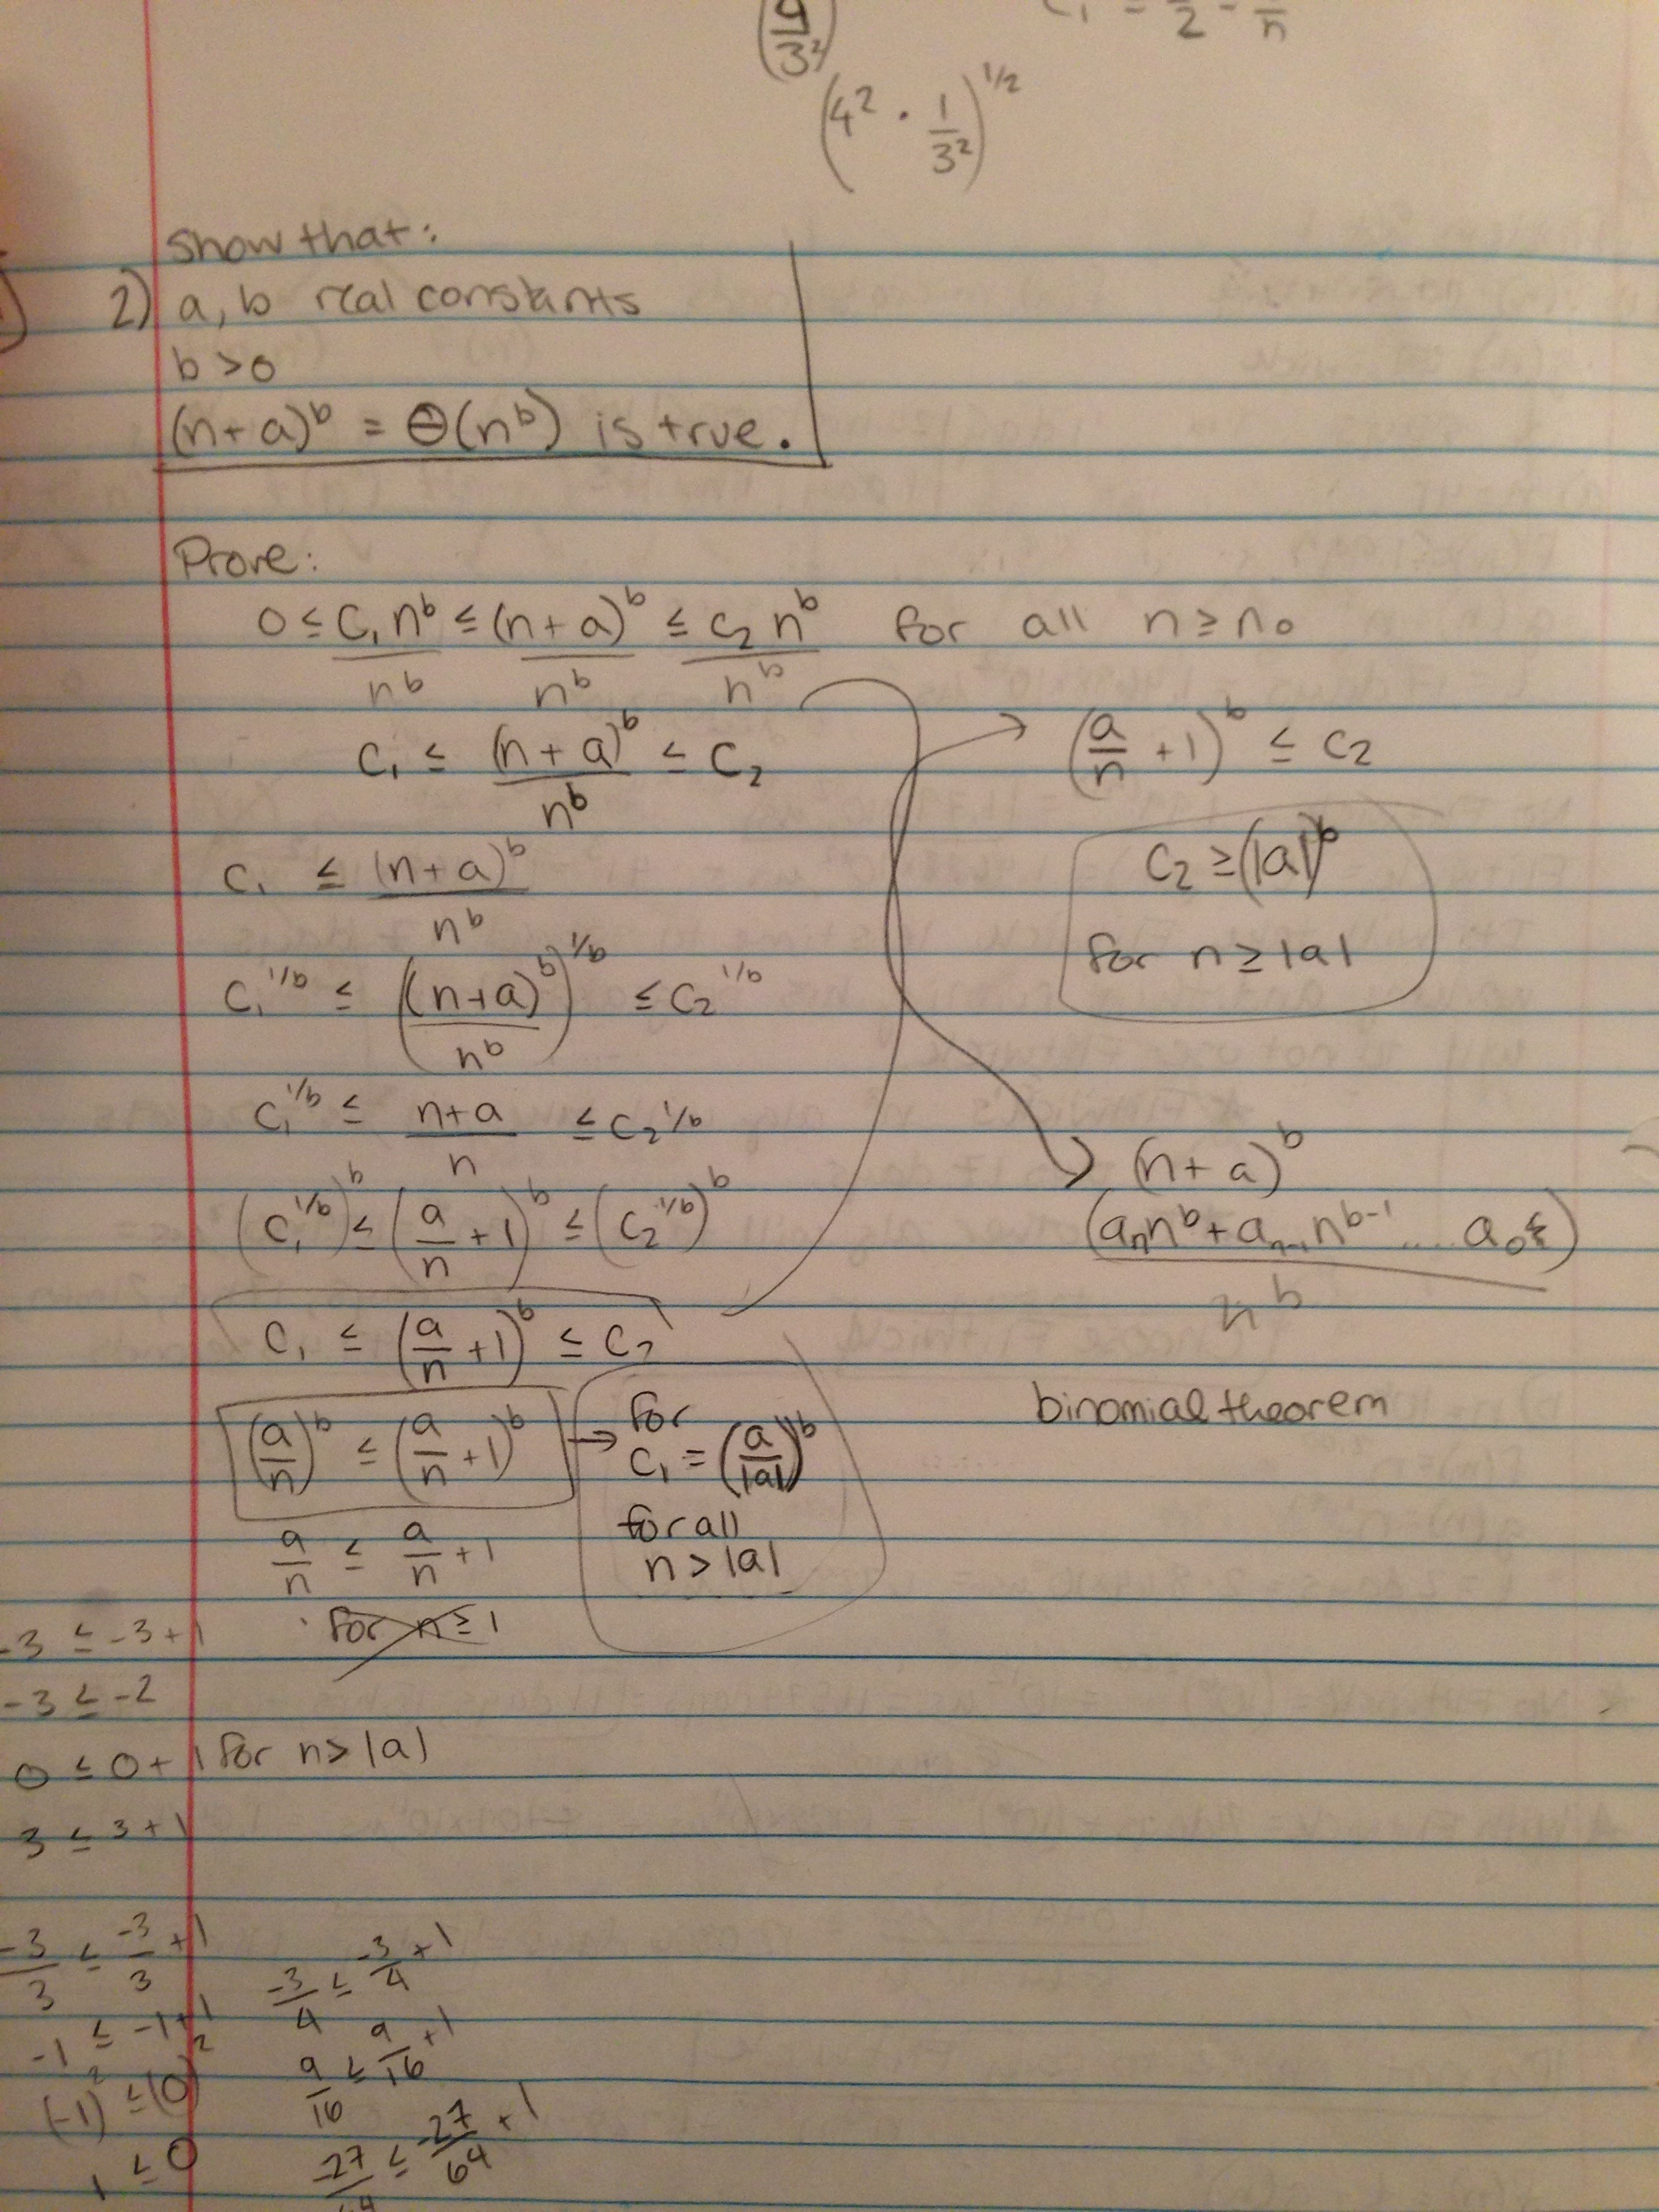
\includegraphics[scale = 1]{problem2.jpg}
\caption{default}
\label{default}
\end{center}
\end{figure}
Another way to look at this problem is that we have\\ $0 \le c_{1}n^{b} \le (n+a)^{b} \le c_{2}n^{b}$ for all $n \ge n^{0}$\\
The series expansion of the $(n+a)^{b}$ numerator  (courtesy of Wolram Alpha) at $n = 0$ is\\ $a^{b}+b n a^{b-1}+1/2 (b-1) b n^{2} a^{b-2}+1/6 (b-2) (b-1) b n^{3} a^{b-3}+1/24 (b-3) (b-2) (b-1) b n^{4} a^{b-4}+O(n^5)$\\\\
We can see that if we divide all sides by $n^{b}$, each term after the first term will be very small as n goes to infinity, leaving a constant relation like $0 \le c_{1} \le A \le c_{2}$ which we can certainly pick $c_{1}$ and $c_{2}$ to satisfy. This insight can be seen in any expansion of a polynomial. The largest term will be an $n^{b}$ term, matching our $\Theta(n^{b})$ as we take the limit as n goes to infinity.\\\\
{\footnotesize I worked on Problem 2 by myself, but I did discuss how we were supposed to prove this with the group Nora Conner, Anshul Kanakia, John Klingner, Andy McEvoy, Bill Casson. We were trying to decide if it makes sense to expand the numerator partially. Since I wasn't sure about that when I did it on my own, and I am also unsure about my other proof, I put both down}
\section{}%3
\subsection{}%a
Is there a c for which $0 \le 2^{nk} \le c2^{n}$  for $ k > 1$?\\\\
Dividing both sides by $2^{n}$:\\
$(2^{n})^{k-1} \le c$\\\\
No. There is no constant c that is greater or equal to $(2^{n})^{k-1}$ for sufficiently large n.
\subsection{}%b
Is there a c for which $0 \le 2^{n+k} \le c2^{n}$  for $ 0 \le k \le c$ (some positive constant)?\\\\
$2^{n}*2^{k} \le c2^{n}$\\
Dividing both sides by $2^{n}$:\\
$2^{k} \le c$for 
Yes. For $n_{o} = 0, c \ge 2^{k}$ where $k \ge 0$.\\\\
{\footnotesize I worked on Problem 3 by myself}
\section{}%4
\subsection{}%a
\begin{figure}[H]
\begin{center}
\includegraphics[scale = 1]{problem4a1.png}
\caption{4a}
\label{default}
\end{center}
\end{figure}
\begin{figure}[H]
\begin{center}
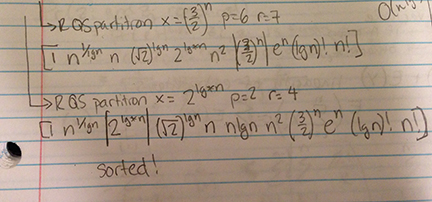
\includegraphics[scale = 1]{problem4a2.jpg}
\caption{4a continued}
\label{default}
\end{center}
\end{figure}

\subsection{}%b
Final order:
$1$, $n^{1/lg n}$, $2^{lg*n}$, $(\sqrt{2})^{lg n}$, $n$, $n lg n$, $lg(n!)$, $n^{2}$, $(3/2)^{n}$, $e^{n}$, $(lg n)!$, $n!$\\\\

Both $n lg n$, $lg(n!)$ are in the $O(n lg n)$ equivalence class.\\\\
{\footnotesize I talked about l'hopitals and comparing some of the functions in 4 with John Klingner, Andy McEvor, and possibly Nora Conner, Anshul Kanakia, and Bill Casson but I don't remember if the latter three really were discussing that problem with us}
\section{}%5
\subsection{}%a
$f_{0} = 3$\\ $f_1 = 5$\\ $f(n) = 3*f_{n-1} - 2*f_{n-2}$ for $n \ge 2$\\ The base cases are f(0) and f(1).
\subsection{}%b
$F_{n} = 3*F_{n-1} - 2*F_{n-2}$\\
$F_{n+2} = 3*F_{n+1} - 2*F_{n}$\\
$F_{n+2} - 3*F_{n+1} + 2*F_{n} = 0$\\
This corresponds to the characteristic polynomial:\\
$x^{2} - 3x + 2 = 0$\\
Solving for the roots:\\
$(x-2)(x-1) = 0$\\
$x = 2$ and $x = 1$\\\\
Using these roots, the expression below solves the recursion:\\
$Fn = a_{1}*2^{n} + a_{2}*1^{n}$\\
To solve for $a_{1}$ and $a_{2}$, we use the two base cases to create a system of equations:\\
$n = 0: 3 = a_{1}*2^{0} + a_{2}*1^{0}$\\
$n = 1: 5 = a_{1}*2^{1} + a_{2}*1^{1}$\\
----------------------------------------- adding the two equations...\\
$-2 = a_{1} - 2*a_{1}$\\
$a_{1} = 2$\\
$a_{2} = 3 - 2 = 1$\\
Therefore:\\
$F_{n} = 2^{n+1} + 1$\\
\subsection{}%c
Base cases: $f(0) = 3 = 2^{0+1} + 1 = 3$ Checks out.\\
$f(1) = 5 = 2^{1+1} + 1 = 5$ Checks out.\\
Assume true up to n-1.\\
$F(n) = 3*F_{n-1} - 2*F_{n-2} = 3*(2^{n-1+1} + 1) - 2*(2^{n-2+1} + 1)$\\
$F(n) = 3*(2^{n} + 1) - 2*(2^{n-1} + 1)$\\
$F(n) = 3*2^{n} + 3 - 2*2^{n-1} - 2$\\
$F(n) = 3*2^{n} - 2^{n}  + 1$\\
$F(n) = 2*2^{n} + 1$\\
$F(n) = 2^{n+1} + 1$ Checks out
\subsection{}%d
$T(n)$ = $\Theta (1)$ if $n \le 1$ and $T(n-1) + T(n-2) + \Theta (1)$ if $n > 1$
\subsection{}%e
The recursion tree of this function will be a height of n and a width of $2^{l}*c$ where c is some constant and l is the level of the recursion tree. A rough integral of the $2^{l}*c$ function over levels (l) from 0 to n shows that the running time would be something like $c2^{n}$. However, the recursion tree is not a dense tree, so it will not actually be reaching the $O(2^{n})$ as a tight bound.
\subsection{}%f
The recurrence relation in (D) can be written as:\\
$T_{0} = c$\\ $T_1 = c$\\ $T(n) = T_{n-1} + T_{n-2} + c$ where the c's are constant times\\
This corresponds to the characteristic polynomial:\\
$x^{2} - x -1 = c$\\
For now, we ignore the constant and solve $x^{2} - x -1 = 0$ for the roots:\\
$x = (1 \pm \sqrt{5})/2$, or the Golden Ratio, $\phi$\\\\
The equations below solve the recursion:
$T(n) = a_{1}*(\phi)^{n} + a_{2}*(1 - \sqrt{5})/2)^{n}$\\
Since we are looking for running time, this corresponds to:\\
$T(n) = O(1.61^{n} - 0.61^{n})$, which explains why $O(2^{n})$ was not a tight bound\\\\
{\footnotesize I worked on problem 5 alone. I did ask about the characteristic polynomials in my study group, but I ended up looking them up and learning them on my own}
\section{}%6
\subsection{}%a
I am assuming that T(0) = 0;
$T(n) = T(n-1) + n$\\
$T(n) = T(n-2) + n-1 + n$\\
$T(n) = T(n-3) + n-2 + n-1 + n$\\
$T(n) = T(n-4) + n-3 + n-2  + n-1 + n$\\
.\\.\\.\\
$T(n) = T(n-(n-1)) + (n-(n-2)) + ... + n-3 + n-2  + n-1 + n$\\
$T(n) = T(n-(n-0)) + T(n-(n-1)) + (n-(n-2)) + ... + n-3 + n-2  + n-1 + n$\\
This leads to:
$T(n) = 0 + n - (n-1) + n -(n-2) + ... + n - (3) + n - (2) + n - (1) + n - (0)$\\
$T(n) = n^{2} - ((n-1) + (n-2) + ... + 3 + 2 + 1)$\\
$T(n) = n^{2} - \sum_{k=1}^{n-1}{k}$\\
$T(n) = n^{2} - (\sum_{k=1}^{n}{k} - n) = n^{2} - (1/2n(n+1) - n)$\\
$T(n) = n^{2} - n^{2}/2 + n/2 - n$\\
$T(n) = n^{2}/2 + n/2$\\
$T(n) = n(n+1)/2$\\
$T(n) = \Theta (n^{2})$
\subsection{}%b
$T(n) = 2T(n/2) + n^{3}$\\
$T(n) = aT(n/b) + f(n)$\\\\
$f(n) = n^{3} = \Omega(n^{log_{b}a + \epsilon})= \Omega(n^{log_{2}2 + \epsilon}) = \Omega(n^{1+\epsilon}) $\\
if $2*f(n) \le cf(n)$\\
$2*(n/2)^{3} \le c*n^3$ for $c < 1$\\
$1/4n^{3} \le cn^{3}$ for $c < 1$\\\\
So, $T(n) = \Theta(n^{3}$
\subsection{}%c
\begin{figure}[H]
\begin{center}
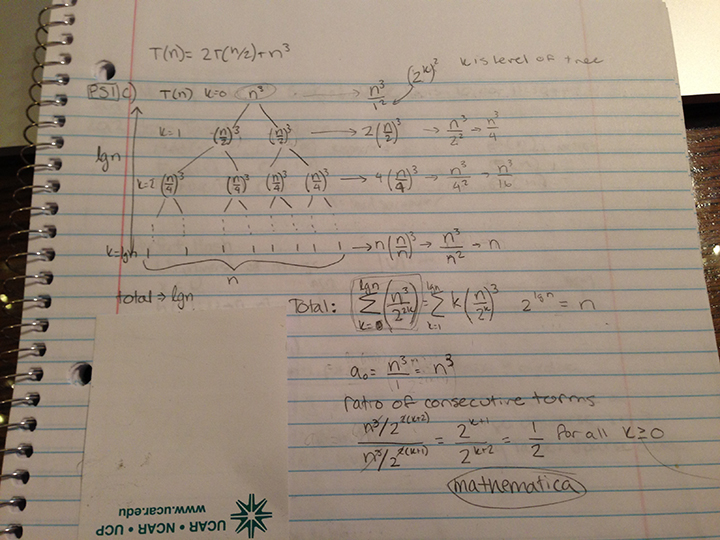
\includegraphics[scale = 0.7]{problem6c.jpg}
\caption{default}
\label{default}
\end{center}
\end{figure}
{\footnotesize Worked alone on problem 6}
\section{}%7
\subsection{}%a
If Snape had n/2 or more 
\subsection{}%b
If there are more than n/2 good chips, then Snape can simply split the n chips in half and compare one set of the chips to the other set. Since over half of them are good, if $n mod 2 = 0$, there must be at least one pair of good chips that get compared to each other. Therefore, he then simply must take one of each Good-Good result to put in his pool to test further against each other in the same manner. The reason he only need to take one of each Good-Good pair is because in a Good-Good outcome, it is possible that both chips are good or both chips are bad. So, there is only a need to try one of the pair, since all that matter is finding one good chip from all the bad ones. In the worst case there is an even number of both bad and good chips, and all the bad chips in the bunch get tested against each other, and they all decided to say that they are Good-Good pairs. So, Snape gets n/2 pairs of Good-Good. This is not a problem, though, because Snape only takes one of each pair of Good-Goods, which will still reduce the size to n/2.

If he continues to follow this pattern, he will quickly keep halving his group of chips.

A key part to this technique is that any time a good chip is paired with a Bad chip, the Good chip prevents the result from being Good-Good. So, bad chips continue to be eliminated any time there is an odd number of bad chips (the extra will be compared to a good chip).

There is also no chance that the Good chips could become outnumbered but he bad chips, because even if all Bad chips are compared to goods, resulting in the elimination of many good chips through Good-Bad pairings, the remaining Good-Good pairs would be only good chips, which would end up getting tested together.
\subsection{}%c
The recurrence relation is $T(n) = 1*T(n/2) + O(n)$ because the problem is split into 1 subset of size $n/2$, and the time it takes to go through the n/2 pairs of results to pick up the one of each Good-Good pair is O(n).

Using the 	Master Method,$ f(n) = O(n) = \Omega(n^{log_{2}(1+0.5)})$ and $1*(n/2) \le c*n$ for $1/2 < c < 1$, $T(N) = \Theta(n)$
\\\\
{\footnotesize I worked on Problem 7 a and b with John Klingner, Andy McEvor, Nora Conner, Anshul Kanakia and a small amount of group discussion was held with Bill Casson. After day one of working with the first 4 in the group, we had not come up with a way to solve B, even though we had recognized pretty easily that A is true. We spent time trying to come up with comparison scenarios. I came up with the final insight on my own after that session, and I discussed it a bit with John Klingner and Anshul Kanakia, since they had said they had solved it too. I hadn't fleshed out the whole solution (ie. picking up only half of the Good-Good pairs) yet, but the hard part was done}
\section{}%8
A smallest possible counterexample is as follows:
\begin{figure}[H]
\begin{center}
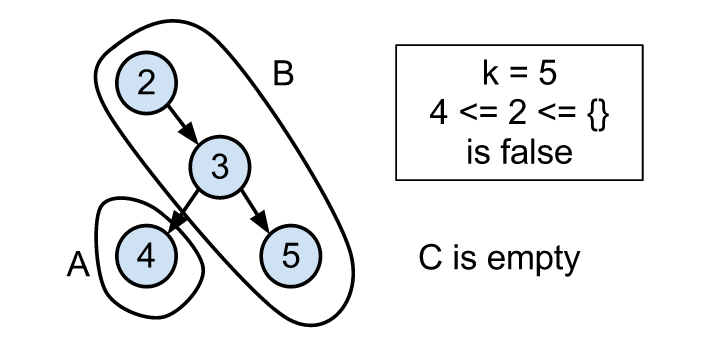
\includegraphics[scale = 0.7]{problem8.png}
\caption{default}
\label{default}
\end{center}
\end{figure}
{\footnotesize I talked about l'hopitals and comparing some of the functions in 4 with John Klingner and Nora Conner, and we looked for examples of binary trees on Wikipedia, which gave good insight. I drew my own tree. Anshul Kanakia, Andy McEvoy, and Bill Casson were working on that problem in the room with the group another day and we did give them a nudge to look for examples. I can't remember if they took it}
\section{}%9
My code is at the end of the file. I am still trying to work out a bug in my insertion code. It is difficult to isolated because it does not happen every time you insert something to the list.
I have implemented Insert, Delete, and Search, but there are still issues.
{\footnotesize Worked alone on problem 9. Did ask Anshul Kanakia if he used arrays or linked lists for the towers and he said that he used linked lists that then were cross-linked}
\section{}%10
Since my SkipList code has bugs for adding things to the list, I was unable to plot the graph.
{\footnotesize Worked alone on problem 9. Did ask Anshul Kanakia if he used arrays or linked lists for the towers and he said that he used linked lists that then were cross-linked}

\section{SOURCE CODE}





\end{document}  